\documentclass{svjour3}                %onecolumn (standard format)
%\documentclass[smallcondensed]{svjour3}     % onecolumn (ditto)
%\documentclass[smallextended]{svjour3}       % onecolumn (second format)
%\documentclass[twocolumn]{svjour3}          % twocolumn
%
\smartqed  % flush right qed marks, e.g. at end of proof
\usepackage{graphicx}
\usepackage{latexsym,bm,amsmath,amssymb}
\usepackage{rotating}
%\usepackage{pdflscape}
\usepackage{multirow,booktabs,cases}
\usepackage[misc]{ifsym}
\usepackage[style=1]{mdframed}
\usepackage{algorithm,algorithmic}
%\usepackage{contour,soul,color}
\usepackage[colorlinks=true]{hyperref}
\hypersetup{urlcolor=blue, citecolor=blue,linkcolor=blue}
\usepackage{epstopdf}
\usepackage{bm}

\def \R {{\mathbb{R}}}
\def \S {{\mathcal{S}}}
\def \I {{\mathcal{I}}}
\def \C {{\mathcal{C}}}
\def \B {{\mathcal{B}}}
\def \X {{\mathcal{X}}}
\def \Y {{\mathcal{Y}}}
\def \Z {{\mathcal{Z}}}
\def \M {{\mathcal{M}}}

\def\argmin{\arg\hspace{-1mm}\min}
\def\argmax{\arg\hspace{-1mm}\max}
\def\lbb{\left\{}
\def\rbb{\right\}}
\def \E {{\mathbb E}}
\def\nn{\nonumber}
\def\st{\hbox{s.t.}}

\newcommand{\lno}{\left\|}
\newcommand{\rno}{\right\|}
\newcommand{\dom}[1]{\mathrm{dom}\,{#1}} %Domain
\newcommand{\inter}[1]{\mathrm{int}\,{#1}} %Interior
\newcommand{\epi}[1]{\mathrm{epi}\,{#1}} %Epigraph
\newcommand{\bd}[1]{\mathrm{bd}\,{#1}} %Boundary
\newcommand{\cl}[1]{\mathrm{cl}\,{#1}} %Closure
\newcommand{\crit}[1]{\mathrm{crit}\,{#1}} % Critical point
\newcommand{\dist}{\mathrm{dist}} %Distance between point and set
\newcommand{\shrink}{\mathrm{shrink}}
\newcommand{\prox}{\mathrm{prox}}
\newcommand{\Proj}{\mathrm{Proj}}
\newcommand{\BP}{\widetilde{P}}



%\usepackage{showkeys} % show the lable in pdf
%\setlength{\textwidth}{\dimexpr\pdfpagewidth-2in}% Equal left/right margins
%\textheight=20cm

%\newtheorem{remark}{{\it Remark}}


%%%%%%%%%%%%%%%%%%%%%Definition for Math Form %%%%%%%%%%%%%%%%%%%%%%%%%%%%%%%%%%%%

%%%%%%%%%%%%%%%%%%%%%%%%%%%%%%%%%%%%%%%%%%%%%%%%%%%%%%%%%%%%%%%%%%%%%%%%%%%%%%%%


\begin{document}
\graphicspath{{./FIG/}}

\title{Bregman generalized subgradient projected algorithms and applications}
\titlerunning{Bregman generalized subgradient projected algorithms and applications}     % if too long for running head

\author{Xiaoyu Mao \and Xianfu Wang}

%\authorrunning{X. Mao\and H. He} % if too long for running head

\institute{X. Mao \and X. Wang \at Department of Mathematics, I.K. Barber Faculty of Science, Kelowna, BC, Canada. \\
\email{alex.mao@ubc.ca}
\and X. Wang (\Letter) \at
\email{shawn.wang@ubc.ca}}


\date{Received: date / Accepted: date}
% The correct dates will be entered by the editor

\maketitle

\begin{abstract}
Projected subgradient methods were thought as ideal algorithms for constrained minimization problems. But they are often hampered by the computational complexity of the projection operator. The Bregman distance has been identified as a potential solution to this issue. The existing mirror descent algorithm, which is designed for one-block constrained minimization problems, has been proved an efficient approach. Previous research has revealed its equivalence with Bregman projected subgradient method. This paper expands the algorithm to two-block situations, thereby increasing its applicability. We also provide its convergence proof. Our algorithm has a strong correlation with another renowned method, the “proximal alternating linearized method,” which can be considered a specific variant of our approach. In the numerical experiments, we choose a variety of examples from various fields. The results consistently indicate that Bregman generalized algorithms significantly reduce computation time, particularly when the variable is constrained to the unit simplex.

\keywords{Bregman distance \and subgradient method \and projection operator \and alternating minimization}
% \PACS{PACS code1 \and PACS code2 \and more}
\subclass{90C29 \and 90C56 }
\end{abstract}

%%%%%%%%%%%%%%%%%%%%%%%%%%%%%%%%%%%%%%
\section{Introduction}\label{Intro}
The two-block minimization problem is an important subset of traditional optimization theory. Numerous practical applications can be abstracted into a two-block problem. For instance, matrix decomposition is a two-block problem, where each factorized matrix corresponds to a block. Sometimes even if the objective function is one-block, we introduce an instrumental variable and a constraint, transforming the problem into a two-block one. It can potentially simplify the process of finding a solution. This paper mainly considers a constrained two-block optimization problem that can be formulated by
\begin{equation}
\begin{aligned} \label{P1}
&\min \quad F(x,y) \quad \st \; x \in \X, y\in \Y, 
\end{aligned}
\end{equation}
where $\X,\Y \subset \R^n$ are closed convex sets, and $F$ satisfies the following assumptions:
\begin{itemize}
  \item $F:\Z=\X\times \Y\rightarrow \overline{\R}$ is partially convex and Lipschitz continuous;
  \item The partial subgradients of $F$ are computable;
  \item The minimizer set $\Z^*$ is nonempty.
\end{itemize}
The subdifferentiability throughout this paper uses Frechet's definition. The partial subdifferentials in the second assumption means that for each fixed point $(z_1,z_2)\in\dom F$, the subdifferentials $\partial_x F(x,z_2)$ and $\partial_y F(z_1,y)$ with respect to $x$ and $y$ in order are easy to compute.

\begin{definition}\label{subdiff}
(Subdifferential) Let $f:\R^m \rightarrow \overline{\R}$ be a proper and lower semicontinuous function
\begin{enumerate}
\item The Frechet subdifferential of function $f$ at $x$, where $x\in \dom f$, denoted by $\hat{\partial} f(x)$, is the collection of all the vectors $u\in\R^m$ which satisfies
\begin{equation}
\lim_{y\neq x,\; \atop y\rightarrow x}\; \inf \; \frac{f(y)-f(x)-\langle u,y-x\rangle}{\|y-x\|} \geq 0.\nn
\end{equation}
When $x\notin \dom f$, otherwise, we let $\hat{\partial} f(x)=\emptyset$.
\item The subdifferential (or limiting subdifferential) is defined through following process
\begin{equation}
\partial f(x)=\{u\in\R^m :\exists y^{\nu}\rightarrow x,f(y^{\nu})\rightarrow f(x) \; {\rm and} \; u^{\nu}\in\hat{\partial} f(y^{\nu})\rightarrow u\}.\nn
\end{equation}
\end{enumerate}
\end{definition}

The partially convexity and Lipschitz continuity are another two fundamental assumptions in this paper. They are defined in the following ways.
\begin{definition}
(Partially convex function) Let $f:\R^m \times \R^n\rightarrow \overline{\R}$ be an extended-real-valued function. Then $f$ is partially convex if $f(\cdot,z_2)$ and $f(z_1,\cdot)$ are two convex functions, i.e. 
\begin{equation*}
f(\alpha x + (1-\alpha)y,z_2)\leq \alpha f(x,z_2) + (1-\alpha)f(y,z_2),
\end{equation*}
for all $x,y\in\dom f(\cdot,z_2)$, and
\begin{equation*}
f(z_1,\alpha x + (1-\alpha)y)\leq \alpha f(z_1,x) + (1-\alpha)f(z_1,y),
\end{equation*}
for all $x,y\in\dom f(z_1,\cdot)$, where $(z_1,z_2)\in\dom f$ is a fixed point and $\alpha\in[0,1]$.
\end{definition}
	
\begin{definition}
(Partially Lipschitz function) Let $f:\R^m \times \R^n \rightarrow \overline{\R}$ be a proper and lower semicontinuous function. Then $f$ is partially Lipschitz if there exists two constants $L_1$ and $L_2$ such that for each fixed point $(z_1,z_2)\in\dom f$, $f(\cdot,z_2)$ and $f(z_1,\cdot)$ are two Lipschitz functions, i.e.
\begin{equation*}
	|f(x,z_2)-f(y,z_2)| \leq L_1 \|x-y\| ,
\end{equation*}
for all $x,y\in \inter \; \dom f(\cdot,z_2)$ and
\begin{equation*}
	|f(z_1,x)-f(z_1,y)|\leq L_2 \|x-y\|,
\end{equation*}
for all $x,y\in \inter \; \dom f(z_1,\cdot)$.
\end{definition}
Note that a partially convex function does not indicate it is convex with respect to the whole blocks. In the other word, partial convexity is weaker than convexity. The similar relation also adopts to Lipschitz continuity. Please refer th following two examples.
\begin{example}
Let $f:\R^m\times\R^n\rightarrow\overline{\R}$ be given by $f(x,y)=f_1(x)f_2(y)$ where $f_1\geq 0$ and $f_2\geq 0$ are two nonnegative convex functions. Then $f$ may be not a convex function but is a partially convex function.
\end{example}
\begin{example}
Let $f:\R^m\times\R^n\rightarrow\overline{\R}$ be $f(x,y)=\langle x,y \rangle$ defined on $\|x\|\leq 1$ and $\|y\|\leq 1$. It is a Lipschitz function with parameter $L=\sqrt{2}$ but a partially Lipschitz function with $L_1=1$ and $L_2=1$.
\end{example}

The conventional approach for solving \eqref{P1} is known as the ``alternating subgradient projected methods'' \cite{L12,SB15}, which is straightforward and efficient. It updates the variables in cyclic order by
\begin{subequations}
\begin{align*}
y^{k+1}&= \Pi_\Y \left( y^k-t_k \hat{g}_k(y^k) \right),\\
x^{k+1}&= \Pi_\X \left( x^k-t_k \hat{h}_k(x^k) \right),
\end{align*}
\end{subequations}
where $\hat{g}_k(y)\in\partial_y F(x_k,y)$ and $\hat{h}_k(x)\in\partial_x F(x,y_{k+1})$ are subgradients, $t_k>0$ are step sizes and $\Pi_{\C}$ is an Euclidean projection onto a closed and nonempty convex set $\C$ defined by $\Pi_\C (x):= \argmin_{y\in \C} \left\{ 1/2\|y-x\|^2 \right\}$. As a gradient (subgradient) based algorithm, it has an oracle complexity independent from the dimension \cite{SB15}. When the decision variable is high dimensional, the convergence rate does not get slower even in high-dimensional settings. This characteristic has led to its widespread application in various fields, including large-scale machine learning and high-dimensional statistics.

Theoretically, this algorithm is suitable for any constrained problems, as long as the projection is well-defined. But in practice, the form of projection operator plays a crucial role and needs to be carefully considered. For simple convex sets, like box (rectangle) sets, affine sets and balls, the computation of the projection operator is relatively straightforward. But for some complicated sets, the form of the projection operator may be implicit. A typical example is unit simplex. In $\R^m$, it is defined by
\begin{equation*}
\S_m:=\left\{ (x_1,x_2,\ldots,x_m) \Big| x_i\geq 0, \sum_{i=1}^m x_i = 1\right\}.
\end{equation*}
Indeed, the calculation of its corresponding Euclidean projection $\Pi_\S$ is challenging. Based on the induction in \cite{CY11} (also see the Appendix), it can be written as
\begin{equation*}
\Pi_{\S_m}(x):=x-\argmin_y \left\{ \max_{1\leq i \leq m}\{y_i\}+\frac{1}{2}\|y-x\|^2 \right\}.
\end{equation*}
Unfortunately, the minimization problem contained in the expression does not have an explicit solution. If applying this projection operator in the subgradient algorithms, we have to solve a nested programming problem at each step $k$. For $\R^m$, the paper \cite{CY11} offers a quick and implementable algorithm to project an arbitrary point onto a unit simplex. The time complexity of this algorithm is primarily determined by the internal ascending sorting procedure. In computer science and combinatorial optimization theory, common sorting algorithms based on swapping, such as quick sort, merge sort, or bucket sort, have a lower-bound time complexity of $m\log(m)$. While there have been proposals for non-swapping or parallel sorting algorithms, the fundamental limitations of sorting algorithms remain challenging to overcome. When dealing with a high-dimensional vector, this procedure can be time-consuming and restricts the performance of algorithms. Our motivation improving the algorithm comes from this issue. We seek to find an better approach to avoid this problem.

The existing mirror descent algorithm offers some inspiration, although it is designed for single-block problems. It enhances the subgradient projected algorithm by applying the concept of Bregman distance. Precisely, they substitute the Euclidean projection operators in the algorithm by Bregman ones. Bregman projections have some exclusive properties that are helpful to computation. For instance, a Bregman projection onto a unit simplex is considerably simpler than a Euclidean one \cite{AM03}. This advantage helps to mitigate the shortcomings of traditional projected methods.

Our contribution is to extend this algorithm to two-block situations and establish the convergence with different assumptions. The paper is organized as the follows:

{\bf Notation:} Throughout this paper, we use $\R^m$ to denote the $m$-dimensional Euclidean space equipped with the inner product defined by $\langle x , y \rangle:=x^{\top}y$. The norm is denoted by $\| \cdot \|$ and the induced dual norm is $\| \cdot \|_*$. The norms most frequently used in this paper are $l_p$ norms defined by $\|x\|_p=\left(\sum_{i=1}^m |x_i|^p\right)^{1/p}$, where $x=(x_1,x_2,\ldots,x_m)$ and $p\geq 1$. When $p=2$, the norm becomes a Euclidean norm $\|x\|_2=\sqrt{\langle x,x \rangle}$. In the rest of the paper, if the type of the norm is not specified, we will default to $\|\cdot\|_2$. The nonnegative orthant is $\R_{+}^m:=\{x\in\R^m|x_i\geq 0, i=1,2,\ldots,m\}$ and the positive orthant is $\R_{++}^m:=\{x\in\R^m|x_i> 0, i=1,2,\ldots,m\}$. More generally, a closed box is denoted by $[a,b]^m:=\{x\in\R^m|a \leq x_i \leq b, i=1,2,\ldots,m\}$ and an open box is denoted by $(a,b)^m:=\{x\in\R^m|a < x_i < b, i=1,2,\ldots,m\}$. The half-open boxes can be represented by $[a,b)^m:=\{x\in\R^m|a \leq x_i < b, i=1,2,\ldots,m\}$
and $(a,b]^m:=\{x\in\R^m|a < x_i \leq b, i=1,2,\ldots,m\}$. Suppose that $\C$ is a set in $\R^m$. The notations $\inter \C$ and $\bd \C$ are the interior and boundary of $\C$. In term of an extended-real-valued, proper and lower semicontinuous function $f:\R^m\rightarrow\overline{\R}=(-\infty,\infty]$ in variational analysis, $\dom f$ and $\epi f$ are its effective domain and epigraph.



\section{Bregman distance and related concepts}
The Bregman distance was initially introduced by L.M. Bregman's paper \cite{B67} in 1967. It is a distance-like function that is nonnegative but usually not symmetric. Similar to a distance, it satisfies a generalized Pythagorean identity. Based on that, it is possible to define a series of concepts, like projection and Pythagorean theorem, and apply them to the algorithms. Bregman distance-based algorithms sometimes exhibit specific advantages compared to the traditional Euclidean distance. An illustrative example is ``mirror descent'' \cite{AM03}, where the Euclidean projection operator in the subgradient projected method is replaced by a Bregman one. When the set associated to the operator is a unit simplex, Bregman projection has a explicit form expression while the Euclidean does not. This characteristic makes mirror decent more efficient than traditional algorithms. In this section, we will introduce in detail.

\subsection{Bregman distance and basic properties}
A Bregman distance is a distance-like function with two input variables associated to a function $\psi:\I\subset\R^m\rightarrow\R$. The formal definition (also see \cite[Chapter 26]{R70}) is
\begin{definition}
(Bregman distance) Let $\psi:\I\rightarrow \R$ be a continuously differentiable and strictly convex function on $\inter \I$ with $\|\nabla \psi(x^k)\|\rightarrow\infty$ for any sequence $\{x^k\}\subset\inter\I\rightarrow\bd \I$ when $k\rightarrow\infty$. Then a function $B_{\psi}:\I \times \inter \I \rightarrow \R$ defined by
\begin{equation*}
	B_{\psi}(x,y)=\psi(x)-\psi(y)-\langle \nabla \psi (y),x-y \rangle,
\end{equation*}
for any $x\in\I$ and $y\in\inter\I$ is called Bregman distance induced by $\psi$, Such a function $\psi$ is also a ``Legendre function'' \cite{BJ97}.
\end{definition}
The function $\psi$ is also called the kernel of Bregman distance sometimes. Since $\psi$ is a convex function, one can verify that $B_{\psi}$ is nonnegative. Another important property is that when $\psi(x)=1/2\|x\|^2$, $B_{\psi}$ reduces to the square of a Euclidean distance. Therefore, $B_{\psi}$ is a generalization of Euclidean distance. But for most other situations, $B_{\psi}$ is not always symmetric, i.e. $B_{\psi}(x,y)\neq B_{\psi}(y,x)$. Similar to triangle inequality for Euclidean distance, Bregman distance also satisfies a relation called the generalized Pythagorean theorem. The proof can be seen in \cite[Lemma 4.1]{AM03}.
\begin{proposition}\label{GPT}
(Generalized Pythagorean theorem) Let $\I\subset\R^m$ be a closed set. If $\psi:\I \rightarrow \R$ is a continuously differentiable function on $\I$, then we have
\begin{equation}
	B_{\psi}(c,a)+B_{\psi}(a,b)-B_{\psi}(c,b)=\langle \nabla \psi (b) - \nabla \psi (a),c-a \rangle,\nn
\end{equation}
for all points $a,b\in \inter \I$ and $c\in \I$.
\end{proposition}

A lot of distance-like functions are actually Bregman distances. They are applied in many fields related to science or engineering used to measure the difference of two objects. The following three examples are just some samples of them.
\begin{example}
(Squared Mahalanobis distance)  When the kernel $\psi_Q(x)=1/2\langle x,Qx \rangle$ is a quadratic function and $\I=\R^m$, where $Q$ is a positive definite matrix, the corresponding Bregman distance $B_{\psi_Q}(x,y)=1/2\langle x-y,Q(x-y) \rangle$ is called squared Mahalanobis distance \cite{M36}. When $Q=I$, it reduces to the squared Euclidean distance.
\end{example}

\begin{example}\label{KL}
(Generalized Kullback–Leibler divergence) When the kernel $\psi_e(x)=\sum_{i=1}^m x_i {\rm log}(x_i)$ is Boltzmann-Shannon entropy and $\I=\R_{+}^m$, the corresponding Bregman distance $B_{\psi_e}(x,y)=\sum_{i=1}^m x_i {\rm log} (x_i/y_i) -\sum_{i=1}^m (x_i - y_i)$ is called generalized Kullback–Leibler (KL) divergence \cite{KL51}. When $x,y\in\S_m$, it turns into Kullback–Leibler divergence.
\end{example}

\begin{example}\label{IS}
(Itakura–Saito distance) When the kernel $\psi_b(x)=-\sum_{i=1}^m {\rm log}(x_i)$ is a Burg’s entropy and $\I=\R_{++}^m$, the corresponding Bregman distance $B_{\psi_b}(x,y)=\sum_{i=1}^m \left( x_i/y_i-{\rm log}(x_i/y_i)-1 \right)$ is called Itakura–Saito distance \cite{IS68}.
\end{example}
Figure \ref{UNIT_BALLS} illustrates intuitively how the Bregman distances differ from Euclidean distance. What appear in the figure are three unit balls centered at $(3,3)$ expressed by $B_{\psi}((x,y),(3,3))=1$. However, it can be observed from the figure that Bregman balls are irregular shapes instead of a circle like Euclidean distance.

\begin{figure}[H]
\centering 
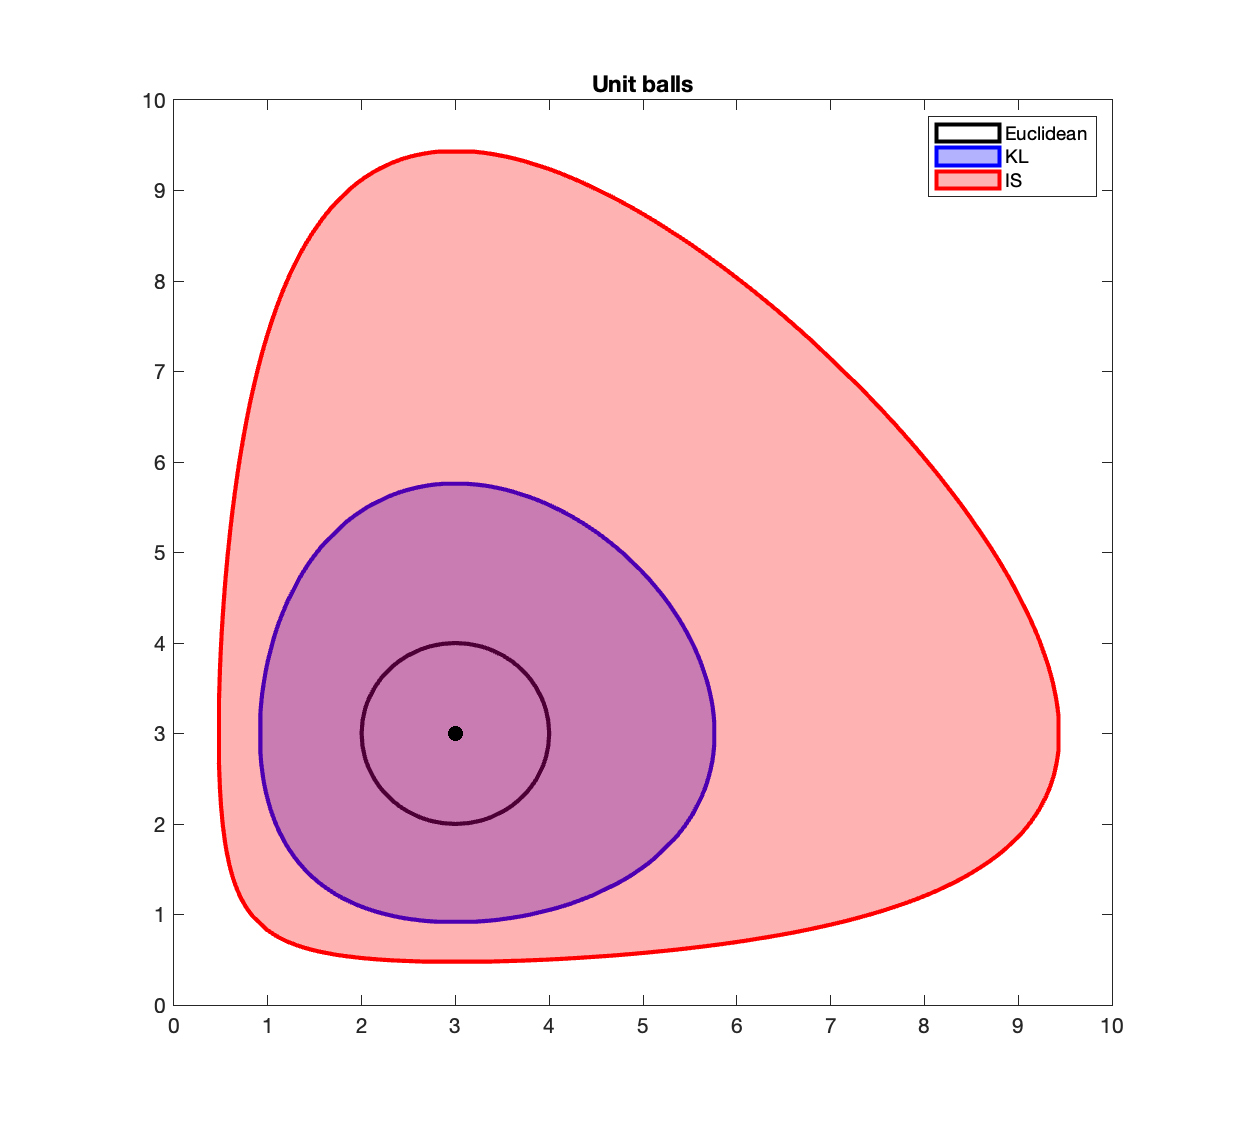
\includegraphics[width=0.65\textwidth]{unit_balls.eps}
\caption{The unit balls in $\R^2$ centered at $(3,3)$ based on Euclidean, Kullback-Leibler and Itakura-Saito distances.}
\label{UNIT_BALLS}
\end{figure}

\subsection{Bregman projection operator}
When we discussed projection operators in the last section, the definition relied on the ``distance'' in a Hilbert space. Now, we extend this concept to a more general situation.
\begin{definition}
(Bregman projection operator) Let $\C\subset \R^m$ be a nonempty and closed convex set. Let $B_{\psi}:\I \times \inter \I \rightarrow \R$ be a Bregman distance. For any $x\in \inter \I$, Bregman projection onto $\C$ is defined by
\begin{equation*}
\widetilde{\Pi}_\C (x):= \argmin_{y\in \C\cap \I}\left\{ B_{\psi} (y,x) \right\}.
\end{equation*}
\end{definition}
Clearly, when $\psi$ is a half squared $l_2$ norm, it reduces to the projection operator under Euclidean distance definition. This type of projection operator is sometimes named ``right Bregman projection operator'' while the left one exchanges the positions of $x$ and $y$ in the Bregman distance.
	

\section*{Acknowledgment}
----------------------------


%\bibliographystyle{spmpsci}
%\bibliography{E:/Research/JabRef/HeArt,E:/Research/JabRef/HeBook,E:/Research/JabRef/Dantzig_Bib}

\begin{thebibliography}{10}
	\providecommand{\url}[1]{{#1}}
	\providecommand{\urlprefix}{URL }
	\expandafter\ifx\csname urlstyle\endcsname\relax
	\providecommand{\doi}[1]{DOI~\discretionary{}{}{}#1}\else
	\providecommand{\doi}{DOI~\discretionary{}{}{}\begingroup
		\urlstyle{rm}\Url}\fi
	
	\bibitem{BJ97}
	H.H. Bauschke and J.M Borwein: Legendre functions and the method of random Bregman projections.
	\newblock Journal of Convex Analysis \textbf{4(1)} 27-67 (1997)
	
	\bibitem{B09}
	H.H. Bauschke, X. Wang, J. Ye and X. Yuan: Bregman distances and Chebyshev sets.
	\newblock Journal of Approximation Theory
	\textbf{159(1)} 3-25 (2009)
	
	\bibitem{HJM17}
	H.H. Bauschke, J. Bolte and M. Teboulle: A descent lemma beyond Lipschitz gradient continuity: first-order methods revisited and applications. 
	\newblock Mathematics of Operations Research
	\textbf{42(2)} 330-348 (2017)
	
	\bibitem{BSS13}
	M.S. Bazaraa, H.D. Sherali and C.M. Shetty: Nonlinear Programming: theory and algorithms.
	\newblock John Wiley and Sons (2013)
	
	\bibitem{AM03}
	A. Beck and M. Teboulle:
	Mirror descent and nonlinear projected subgradient methods for convex optimization.
	\newblock Operations Research Letters \textbf{31(3)} 167-175 (2003)
	
	\bibitem{AL13}
	A. Beck and L. Tetruashvili: On the convergence of block coordinate descent type methods. 
	\newblock SIAM Journal on Optimization
	\textbf{23(4)} 2037-2060 (2013)
	
	\bibitem{A17}
	A. Beck: First-order methods in optimization.
	\newblock Society for Industrial and Applied Mathematics (2017)
	
	\bibitem{BTN01}
	A. Ben-Tal, T. Margalit and A. Nemirovski: The ordered subsets mirror descent optimization method with applications to tomography.
	\newblock SIAM Journal on Optimization 
	\textbf{12(1)} 79-108 (2001)
	
	\bibitem{B99}
	D.P. Bertsekas: Nonlinear Programming, 2nd Ed.
	\newblock Athena Scientific, Belmont (1999)
	
	\bibitem{BSM14}
	J. Bolte, S. Sabach and M. Teboulle: Proximal alternating linearized minimization for nonconvex and nonsmooth problems. 
	\newblock Mathematical Programming 
	\textbf{146(1)} 459-494 (2014)
	
	\bibitem{SV04}
	S. Boyd and L. Vandenberghe: Convex Optimization.
	\newblock Cambridge University Press (2004)
	
	\bibitem{B67}
	L.M. Bregman: The relaxation method of finding the common point of convex sets and its application to the solution of problems in convex programming
	\newblock USSR Computational Mathematics and Mathematical Physics
	\textbf{7(3)}, 200-217 (1967)
	
	\bibitem{SB15}
	S. Bubeck: Convex Optimization: Algorithms and Complexity.
	\newblock Foundations and Trends® in Machine Learning (2015)
	
	\bibitem{M36}
	M.P. Chandra: On the generalised distance in statistics.
	\newblock Proceedings of the National Institute of Sciences of India
	\textbf{2(1)} (1936)
	
	\bibitem{CY11}
	Y. Chen and X. Ye: Projection onto a simplex. 
	\newblock arXiv preprint arXiv:1101.6081 (2011)
	
	\bibitem{D51}
	G.B. Dantzig: Maximization of a linear function of variables subject to linear inequalities.
	\newblock Activity Analysis of Production and Allocation
	\textbf{13} 339-347 (1951)
	
	\bibitem{D67}
	I.I. Dikin: Iterative solution of problems of linear and quadratic programming.
	\newblock Doklady Akademii Nauk
	\textbf{174(4)} (1967)
	
	\bibitem{CT07}
	C. Emmanuel and T. Tao: The Dantzig selector: Statistical estimation when $p$ is much larger than $n$. 
	\newblock The Annals of Statistics
	\textbf{35(6)} 2313-2351 (2007)
	
	\bibitem{GKZ18}
	B.R Gaines, J. Kim and H. Zhou: Algorithms for fitting the constrained lasso.
	\newblock Journal of Computational and Graphical Statistics
	\textbf{27(4)} 861-871 (2018)
	
	\bibitem{IS68}
	F. Itakura and S. Saito: Analysis synthesis telephony based on the maximum likelihood method.
	\newblock Reports of the 6th International Congress on Acoustics (1968)
	
	\bibitem{KS12}
	C. Kan and W. Song: The Moreau envelope function and proximal mapping in the sense of the Bregman distance.
	\newblock Nonlinear Analysis: Theory, Methods and Applications 
	\textbf{75(3)} 1385-1399 (2012)
	
	\bibitem{KB09}
	T.G. Kolda and B.W. Bader: Tensor decompositions and applications.
	\newblock SIAM Review
	\textbf{51(3)} 455-500 (2009)
	
	\bibitem{KL51}
	S. Kullback and R.A. Leibler: On information and sufficiency.
	\newblock The Annals of Mathematical Statistics
	\textbf{22(1)} 79-86 (1951)
	
	\bibitem{Y89}
	Y. LeCun et al: Backpropagation applied to handwritten zip code recognition.
	\newblock Neural Computation
	\textbf{1(4)} 541-551 (1989)
	
	\bibitem{L12}
	C. Lemaréchal: Cauchy and the gradient method. 
	\newblock Documenta Mathematica Extra Volume
	\textbf{251(254)}  10 (2012)
	
	\bibitem{LPZ12}
	Z. Lu, T.K. Pong and Y. Zhang: An alternating direction method for finding Dantzig selectors. 
	\newblock Computational Statistics and Data Analysis
	\textbf{56(12)} 4037-4046 (2012)
	
	\bibitem{NH10}
	V. Nair and G.E. Hinton: Rectified linear units improve restricted Boltzmann machines. 
	\newblock ICML (2010)
	
	\bibitem{A14}
	A. Nitanda: Stochastic proximal gradient descent with acceleration techniques. \newblock Advances in Neural Information Processing Systems
	\textbf{27} (2014)
	
	\bibitem{D14}
	D. Noll: Convergence of non-smooth descent methods using the Kurdyka–Łojasiewicz inequality.
	\newblock Journal of Optimization Theory and Applications
	\textbf{160(2)} 553-572 (2014)
	
	\bibitem{P14}
	P. Ochs, Y. Chen, T. Brox and T. Pock: iPiano: Inertial proximal algorithm for nonconvex optimization.
	\newblock SIAM Journal on Imaging Sciences
	\textbf{7(2)} 1388-1419 (2014)
	
	\bibitem{R70}
	R.T. Rockafellar. Convex Analysis. 
	\newblock Princeton University Press, New Jersey (1970)
	
	\bibitem{RW98}
	R.T. Rockafellar and R. J.-B. Wets: Variational Analysis. 
	\newblock Springer, New York (1998)
	
	\bibitem{RM16}
	R. Shefi and M. Teboulle: On the rate of convergence of the proximal alternating linearized minimization algorithm for convex problems. 
	\newblock EURO Journal on Computational Optimization
	\textbf{4(1)} 27-46 (2016)
	
	\bibitem{T96}
	R. Tibshirani: Regression shrinkage and selection via the lasso.
	\newblock Journal of the Royal Statistical Society: Series B (Methodological)
	\textbf{58(1)} 267-288 (1996)
	
	\bibitem{T05}
	R. Tibshirani, M. Saunders, S. Rosset, J. Zhu and K. Knight: Sparsity and smoothness via the fused lasso.
	\newblock Journal of the Royal Statistical Society: Series B (Statistical Methodology) 
	\textbf{67(1)} 91-108 (2005)
	
	\bibitem{T11}
	R.J. Tibshirani and J. Taylor: The solution path of the generalized lasso.
	\newblock The Annals of Statistics
	\textbf{39(3)} 1335-1371 (2011)
	
	\bibitem{T01}
	P. Tseng: Convergence of a block coordinate descent method for nondifferentiable minimization. 
	\newblock Journal of optimization theory and applications
	\textbf{109(3)} 475 (2001)
	
	\bibitem{CG96}
	C.F. Van Loan and G. Golub: Matrix Computations.
	\newblock Johns Hopkins Studies in Mathematical Sciences (1996)
	
	\bibitem{ONF22}
	O. Vu-Thanh, N. Gillis and F. Lecron: Bounded Simplex-Structured Matrix Factorization.
	\newblock ICASSP 2022-2022 IEEE International Conference on Acoustics, Speech and Signal Processing (2022)
	
	\bibitem{YY12}
	Y. Wang and Y. Zhang: Nonnegative matrix factorization: A comprehensive review. 
	\newblock IEEE Transactions on Knowledge and Data Engineering
	\textbf{25(6)} 1336-1353 (2012)
	
	\bibitem{WS15}
	S. Wright: Coordinate descent algorithms. 
	\newblock Mathematical Programming
	\textbf{151(1)} 3-34 (2015)
	
	\bibitem{YW13}
	Y. Xu and W. Yin: A block coordinate descent method for regularized multiconvex optimization with applications to nonnegative tensor factorization and completion.
	\newblock SIAM Journal on Imaging Sciences
	\textbf{6(3)} 1758-1789 (2013)
	
	\bibitem{YL06}
	M. Yuan and Y. Lin: Model selection and estimation in regression with grouped variables.
	\newblock Journal of the Royal Statistical Society: Series B (Statistical Methodology)
	\textbf{68(1)} 49-67 (2006)
	
	\bibitem{HT05}
	H. Zou and T. Hastie: Regularization and variable selection via the elastic net. \newblock Journal of the Royal Statistical Society: series B (Statistical Methodology) 
	\textbf{67(2)} 301-320 (2005)
	
	\bibitem{Y17}
	Y. Zhu: An augmented ADMM algorithm with application to the generalized lasso problem.
	\newblock Journal of Computational and Graphical Statistics
	\textbf{26(1)} 195-204 (2017)
	  
	
\end{thebibliography}



\end{document}

